\documentclass[12pt,letterpaper,fleqn]{article}
\usepackage{fullpage}
\usepackage[top=2cm, bottom=4.5cm, left=2.5cm, right=2.5cm]{geometry}
\usepackage{amsmath,amsthm,amsfonts,amssymb,amscd}
\usepackage[utf8]{inputenc}
\usepackage{lastpage}
\usepackage{enumerate}
\usepackage{fancyhdr}
\usepackage{mathrsfs}
\usepackage{xcolor}
\usepackage{graphicx}
\usepackage{listings}
\usepackage{hyperref}
\usepackage{amsmath}
\usepackage{nccmath}
\usepackage{physics}

\newcommand{\R}{\mathbb{R}}
\newcommand{\Q}{\mathbb{Q}}

\newcommand{\cent}{$^{\circ}$}
\newcommand{\delfrac}[2][y]{\frac{\partial #1}{\partial #2}}


\hypersetup{%
 colorlinks=true,
  linkcolor=blue,
  linkbordercolor={0 0 1}
}
 
\renewcommand\lstlistingname{Algorithm}
\renewcommand\lstlistlistingname{Algorithms}
\def\lstlistingautorefname{Alg.}

\lstdefinestyle{Python}{
    language        = Python,
    frame           = lines, 
    basicstyle      = \footnotesize,
    keywordstyle    = \color{blue},
    stringstyle     = \color{green},
    commentstyle    = \color{red}\ttfamily
}

\setlength{\parindent}{0.3in}
\setlength{\parskip}{0.05in}

% Edit these as appropriate
\newcommand\course{Física - Frente 1}
\newcommand\hwnumber{1}                  % <-- homework number
\newcommand\NetIDa{netid19823}           % <-- NetID of person #1
\newcommand\NetIDb{netid12038}           % <-- NetID of person #2 (Comment this line out for problem sets)

\pagestyle{fancyplain}
\headheight 35pt
%\lhead{\NetIDa}
%\lhead{\NetIDa\\\NetIDb}                 % <-- Comment this line out for problem sets (make sure you are person #1)
\chead{\textbf{\Large Leis de Newton \hwnumber}}
\rhead{\course \\ Maio/2020}
\lfoot{}
\cfoot{}
\rfoot{\small\thepage}
\headsep 1.5em

\begin{document}
\begin{enumerate}
    \item Um paraquedista salta de um avião e cai em queda livre até sua velocidade de queda se tornar constante. Podemos afirmar que a força total atuando sobre o pára-quedista após sua velocidade se tornar constante é:
    \begin{enumerate}
        \item vertical e para baixo. 
        \item vertical e para cima. 
        \item nula
        \item horizontal e para a direita.
        \item horizontal e para a esquerda
    \end{enumerate}
    
    \item Uma caixa encontra-se sobre um plano horizontal e sobre ela uma força constante de intensidade u atua horizontalmente da esquerda para a direita, garantindo-lhe um movimento retilíneo e uniforme. Com base nas leis de Newton, analise:
    \begin{figure}[h]
        \centering
        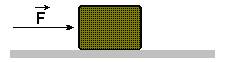
\includegraphics[width=0.5\textwidth]{ex_2.jpg}
    \end{figure}
    \begin{enumerate}[I]
        \item Uma pessoa, dentro da caixa e impedida de ver o exterior, teria dificuldade em afirmar que a caixa possui movimento relativamente ao plano horizontal.
        \item A força resultante sobre a caixa é um vetor horizontal, que possui sentido da esquerda para a direita e intensidade igual a u.
        \item O componente do par ação/reação correspondente à força F é outra força que atua sobre a caixa, horizontalmente, com a mesma intensidade de u, porém de sentido da direita para a esquerda.
    \end{enumerate}
    Está correto o contido em:
    \begin{enumerate}
        \item I
        \item II
        \item I e II 
        \item II e III
        \item I, II e III
    \end{enumerate}
    
    \item  “Excelentes cavaleiros eram os indígenas pampeanos (charruas, minuanos, etc.) que se destacavam na montaria de cavalos vindos da Europa". Um pampeano é lançado para a frente quando o cavalo, assustado com uma cobra, pára de repente. O fato de o indígena não parar ao mesmo tempo que o cavalo pode ser atribuído a seu(sua):
    \begin{enumerate}
        \item Impulso
        \item Peso
        \item Altura
        \item Massa
        \item Força
    \end{enumerate}
    
    \item Uma das modalidades esportivas em que nossos atletas têm sido premiados em competições olímpicas é a de barco a vela. Considere uma situação em que um barco de 100 kg, conduzido por um velejador com massa de 60 kg, partindo do repouso, se desloca sob a ação do vento em movimento uniformemente acelerado, até atingir a velocidade de 18 km/h. A partir desse instante, passa a navegar com velocidade constante. Se o barco navegou 25 m em movimento uniformemente acelerado, qual é o valor da força aplicada sobre o barco? Despreze resistências ao movimento do barco.
    
    \textit{Dica: Caso precise, a conversão km/h $\rightarrow$ m/s é dividir a velocidade por 3,6. Primeiramente encontre a aceleração do barco no MUV (detalhe: talvez não precise achar o tempo!). Depois encontre a força.}
    
    \item Analise a afirmativa a seguir: Em uma colisão entre um carro e uma moto, ambos em movimento e na mesma estrada, mas em sentidos contrários, observou-se que após a colisão a moto foi jogada a uma distância maior do que a do carro.

Baseado em seus conhecimentos sobre mecânica e na análise da situação descrita acima, bem como no fato de que os corpos não se deformam durante a colisão, é correto afirmar que, durante a mesma,

\begin{enumerate}
    \item A força de ação é menor do que a força de reação, fazendo com que a aceleração da moto seja maior que a do carro, após a colisão, já que a moto possui menor massa.
    \item A força de ação é maior do que a força de reação, fazendo com que a aceleração da moto seja maior que a do carro, após a colisão, já que a moto possui menor massa.
    \item As forças de ação e reação apresentam iguais intensidades, fazendo com que a aceleração da moto seja maior que a do carro, após a colisão, já que a moto possui menor massa.
    \item A força de ação é menor do que a força de reação, porém a aceleração da moto, após a colisão, depende das velocidades do carro e da moto imediatamente anteriores a colisão.
    \item Exercerá maior força sobre o outro aquele que tiver maior massa e, portanto, irá adquirir menor aceleração após a colisão.
\end{enumerate}

\item Certo carro nacional demora 30 s para acelerar de 0 a 108 km/h. Supondo sua massa igual a 1200 kg, o módulo da força resultante que atua no veículo durante esse intervalo de tempo é, em N, igual a:

\textit{Note e adote: km/h $\rightarrow$ m/s: /3,6}

\begin{enumerate}
    \item 0 N
    \item 1200 N
    \item 3600 N
    \item 4320 N
    \item 36000 N
\end{enumerate}

\item Usado para missões suborbitais de exploração do espaço, o VS-30, foguete de sondagem brasileiro, possui massa total de decolagem de, aproximadamente, 1 500 kg e seu propulsor lhe imprime uma força de $95.10^3$ N. Supondo que um desses foguetes seja lançado verticalmente em um local onde a aceleração da gravidade tem valor 10 m/s$^2$, desconsiderando a gradual perda de massa devido à combustão, a aceleração imprimida ao conjunto nos instantes iniciais de sua ascensão, relativamente ao solo, é, aproximadamente, em m/s$^2$:
\begin{enumerate}
    \item 15
    \item 24
    \item 36
    \item 42
    \item 53
\end{enumerate}

\item A respeito das leis de Newton, são feitas três afirmativas:
\begin{enumerate}[I]
    \item A força resultante necessária para acelerar, uniformemente, um corpo de massa 4,0kg, de 10m/s para 20m/s, em uma trajetória retilínea, em 5,0s, tem módulo igual a 8,0N.
    \item Quando uma pessoa empurra uma mesa, ela não se move, podemos concluir que a força de ação é anulada pela força de reação. 
    \item Durante uma viagem espacial, podem-se desligar os foguetes da nave que ela continua a se mover. Esse fato pode ser explicado pela primeira lei de Newton.
\end{enumerate}
As afirmações corretas são:

\begin{enumerate}
    \item Todas
    \item Nenhuma
    \item Somente I e II
    \item Somente I e III
    \item Somente II e III
\end{enumerate}

\item Um pescador possui um barco a vela que é utilizado para passeios turísticos. Em dias sem vento, esse pescador não conseguia realizar seus passeios.  Tentando superar tal dificuldade, instalou, na popa do barco, um enorme ventilador voltado para a vela, com o objetivo de produzir vento artificialmente. Na primeira oportunidade em que utilizou seu invento, o pescador percebeu que o barco não se movia como era por ele esperado. O invento não funcionou!

A razão para o não funcionamento desse invento é que
\begin{enumerate}
    \item A força de ação atua na vela e a de reação, no ventilador.
    \item A força de ação atua no ventilador e a de reação, na água.
    \item Ele viola o princípio da conservação da massa. 
    \item As forças que estão aplicadas no barco formam um sistema cuja resultante é nula.
    \item Ele não produziu vento com velocidade suficiente para movimentar o barco.
\end{enumerate}

\item Uma carreta com 4,4 m de comprimento se move com velocidade constante de 12 m/s, até bater numa parede,
parando de modo brusco. Uma pequena caixa de metal, com massa de 3,0 kg, colocada sobre a carreta (ver figura), move-se solidariamente com esta até o momento da batida.

\begin{figure}[h]
    \centering
    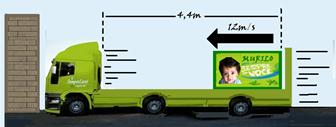
\includegraphics[width=0.6\textwidth]{ex_10.jpg}
\end{figure}

Imediatamente após a batida, a caixa desliza sobre a carreta, movendo-se na direção da parede e sofrendo a ação de uma força de atrito horizontal constante e igual a 15 N. A velocidade de impacto da caixa contra a parede, em m/s, é:
\begin{enumerate}
    \item 8
    \item 9
    \item 10
    \item 11
    \item 12
\end{enumerate}

\item Um automóvel movendo-se em uma BR, guiado por um aluno de física, falta combustível ao se aproximar de um posto de gasolina. Lembrando-se de uma aula sobre o princípio de ação e reação, ele raciocinou: “se eu descer do carro e tentar empurrá-lo com uma força $\Vec{F}$, ele vai reagir com uma força –$\Vec{F}$ e ambas vão se anular e eu não conseguirei mover o carro”. Mas uma pessoa que vinha com ele, não concordando com este raciocínio, desceu do carro e o empurrou, conseguindo movê-lo. Como você justificaria o carro mover-se?

Com base na compreensão desta lei, analise as proposições a seguir.

\begin{enumerate}[I]
    \item O carro move-se porque a pessoa dá um rápido empurrão no carro e, momentaneamente, essa força é maior do que a força que o carro exerceu sobre ela.
    \item O carro move-se porque a pessoa empurra o carro para frente com uma força maior do que a força com que o carro exerce sobre ela.
    \item O carro move-se porque a força que a pessoa exerce sobre o carro é tão intensa quanto a que o carro exerce sobre ela, no entanto, a força de atrito que a pessoa exerce (entre os pés e o solo) é grande e é para frente, enquanto a que ocorre no carro (entre os pneus e solo) é pequena e para trás.
    \item O carro move-se porque a força que a pessoa exerce sobre o carro e a força que o carro exerce sobre a pessoa são iguais, de sentidos contrários, mas aplicados em corpos diferentes e, portanto, cada um exerce o seu efeito independentemente.
\end{enumerate}
A partir da análise feita, assinale a alternativa correta:
\begin{enumerate}
    \item Apenas a IV
    \item As proposições III e IV.
    \item As proposições I e III.
    \item As proposições II e III.
    \item As proposições II e IV.
\end{enumerate}
\item Um pequeno automóvel colide frontalmente com um caminhão cuja massa é cinco vezes maior que a massa do automóvel. Em relação a essa situação, marque a alternativa que contém a afirmativa correta.
\begin{enumerate}
    \item Ambos experimentam desaceleração de mesma intensidade.
    \item Ambos experimentam força de impacto de mesma intensidade.
    \item O caminhão experimenta desaceleração cinco vezes mais intensa que a do automóvel.
    \item O automóvel experimenta força de impacto cinco vezes mais intensa que a do caminhão.
    \item O caminhão experimenta força de impacto cinco vezes mais intensa que a do automóvel.
\end{enumerate}
\end{enumerate}
\newpage
\section*{GABARITO}
\begin{enumerate}
    \item (c)
    \item (a) - porque se o movimento é uniforme e retílineo, não há aceleração, logo a força resultante é 0. Assim o item II está errado. O par ação/reação só acontece quando um corpo aplica uma força no outro corpo. Aqui temos somente uma força aplicada em um corpo, logo o item III está errado. O item I está certo, porque nós só sentirmos a aceleração (a pressão no peito quando o carro acelera e a pressão do cinto de segurança no peito quando o carro freia.), então não sentimos se estamos ou não em movimento.
    
    \item (a) - o que faz o cavaleiro(a) continuar indo para frente mesmo quando o cavalo para é devido à inércia. Como a medida da inércia é a massa, então é a letra (c).
    \item $F = 80\,N$
    
    \item (c) - o par de forças ação e reação tem a mesma intensidade. Com isso, a moto foi jogada a uma distância maior, porque a massa dela é menor que a do carro, portanto a aceleração sofrida pela moto é maior, fazendo ela ser jogada mais longe.
    
    \item (b)
    
    \item (e)
    
    \item (d) - porque o par ação/reação não acontecem no mesmo corpo, ocorrem em corpos diferentes. Então, elas nunca se anulam, logo II está incorreta.
    
    \item (d) - O ventilador empurra o ar para frente, enquanto a vela empurra o ar para trás, para frear o ar. Como os dois estão no barco, então esse par de forças tem direções opostas e se cancelam. 
    
    \item (c)
    
    \item (a)
    
    \item (b)
\end{enumerate}
\end{document}
